\documentclass[a4paper,11pt]{article}

\usepackage[utf8]{inputenc}

\usepackage{graphicx}
\usepackage{caption}
\usepackage{subcaption}

\usepackage{pgfplots}
\pgfplotsset{compat=1.18} 

\usepackage{minted}
\usepackage{siunitx}

\begin{document}

\title{
    \textbf{Performance of Array Operations in C}
}
\author{Mo Wang}
\date{Spring 2026}

\maketitle

\section*{Introduction}

This report investigates the performance in terms of elapsed time of three array operations in C: random access of element, linear search of an element, and searching for duplicated elements in an array. As an introduction to algorithm and data structure, the purpose is to understand algorithms behavior such as time consumption in practice by measuring the elapsed time of each operation in arrays of different sizes. 

\section*{Benchmarking}

For timing a function, the clock \texttt{CLOCK\_MONOTONIC} in C is used. The start and end time are timed using the function \texttt{clock\_gettime} that writes to variables \texttt{t\_start} as start time and \texttt{t\_end}, which are passed as pointer arguments.

The function \texttt{nano\_seconds} takes in the variables textt{t\_start} as start time and \texttt{t\_end} as pointers to \texttt{struct timespec} and calculate a time difference in nanoseconds in \\textt{long} type.

\begin{minted}[breaklines]{C}
  long nano_seconds(struct timespec *t_start, struct timespec *t_stop) {
      return (t_stop->tv_nsec- t_start->tv_nsec) + (t_stop->tv_sec- t_start->tv_sec)*1000000000;
  }
\end{minted}

 The example is shown for benchmarking random array accessing.

\begin{minted}[breaklines]{C}
  // Initial the variable int array[] and index_array[]
  struct timespec t_start, t_stop;
  int sum = 0;
     
  clock_gettime(CLOCK_MONOTONIC, &t_start);
  for (int i = 0; i < loop; i++){
    sum += array[index_array[i]]; // Algorithm operation
  }
  clock_gettime(CLOCK_MONOTONIC, &t_stop);

  long elapsed_time = nano_seconds(&t_start, &t_stop);
  // return elapsed time of batch benchmark
\end{minted}

However, clock precision for timing an algorithm is limited. This is mainly due to the limited clock precision of \texttt{CLOCK\_MONOTONIC} in C from the POSIX \texttt{time.h} header, usually in orders of hundreds of nanoseconds. Because of that, timing individual operations does not produce precise measurements and is thus unreliable, especially timing array access operation in orders of nanoseconds. To mitigate this issue, the same algorithm is executed over again multiple times, in my case 1024 times, while being batch timed. An average time can be calculated for estimating each amortized elapsed time for one individual operation.

Besides, the elapsed time differ in different computing systems and can also fluctuate when using the same computing system. Multiple factors can interfere with execution time, including hardware constraints, operating system time scheduler and background processes. To address this issue, same performance benchmark test is repeated a number of times, while an average elapsed time among the test result is calculated, in order to gain more accuracy.

The code for the benchmark is shown as below for random array access benchmark using the function \texttt{random\_access\_benchmark}:

\begin{minted}[breaklines]{C}
  int main(int argc, char *argv[]) {
      int SIZE_LENGTH = 8;
      int sizes[] = {1024, 2048, 4096, 8192, 16384, 32768, 65536, 131072};
      int trials = 16;
      int loop = 1024;
      for (int i = 0; i < SIZE_LENGTH; i++) {
          int size = sizes[i];
          long min = LONG_MAX;
          long max = 0;
          long total = 0;
          
          printf("--- BENCHMARK MEASUREMENTS (%d, %d SIZE) ---\n", i, size);
          for (int j = 0; j < trials; j++) {
              long elapsed_time = random_access_benchmark(size, loop);
              if (elapsed_time < min){
                  min = elapsed_time;
              }
              if (elapsed_time > max){
                  max = elapsed_time;
              }
              total += elapsed_time;
              printf("ELAPSED TIME: TOTAL: %ld ns, AVG PER LOOP: %0.2f ns\n", elapsed_time, (double) elapsed_time/loop);
          }
          printf("\n");
      
          printf("--- BENCHMARK SUMMARY (%d) ---\n", i);
          printf("MAX TIME: %.2f ns/operation \n", (double)max/loop);
          printf("MIN TIME: %.2f ns/operation \n", (double)min/loop);
          printf("AVG TIME: %.2f ns/operation \n", (((double)total)/loop)/trials);
          printf("TOT TIME: %.2f ns/operation \n", (((double)total)/loop));
          printf("\n\n");
      }
      return 0;
  }
\end{minted}

In order to avoid compiler to optimize away performance benchmark code as dead code, the results of each operation are accumulated into a variable and read after the benchmark test loops. All arrays are allocated on the heap and initially filled with pseudo-random numbers in order to avoid cache locality and further optimizations that can obscure testing. For each benchmark, the array size is double as large as the previous one, in order to calculate a relevant scaling behavior and growth trend in a growing array size.

Finally, the reported numbers use an appropriate number of digits. The goal with the three benchmarks is not to claim unrealistic and arbitrary precision, but to illustrate clear performance trends as the input size increases.

\section*{Random access}

In order to measure the elapsed time of random array access, an index array \texttt{index\_array} is first constructed and filled with pseudo-random indices. During the benchmark, each element of \texttt{index\_array} is used to access the corresponding element of the array \texttt{array}, measuring the time required for random access operations while excluding the random number generation delay.

\begin{minted}[breaklines]{C}
  long random_access_benchmark(int n, int loop) {
      srand(time(NULL)); // set the random seed
      int *array = malloc(n * sizeof(int));
      int *index_array = malloc(loop * sizeof(int));

      // fill array and index_array
      for (int i = 0; i < n; i++){
          array[i] = i;
      }
      for (int i = 0; i < loop; i++){
          index_array[i] = rand() % n;
      }
  
      struct timespec t_start, t_stop;
      int sum = 0;
  
      clock_gettime(CLOCK_MONOTONIC, &t_start);
      for (int i = 0; i < loop; i++){
          sum += array[index_array[i]];
      }
      clock_gettime(CLOCK_MONOTONIC, &t_stop);
  
      free(array);
      free(index_array);
      
      // Force compiler to not let sum variable and its operation be treated as dead code
      if (sum == 0){
          return 0;
      }
      return nano_seconds(&t_start, &t_stop);
  }
\end{minted}

In Table 1, where the benchmark results are shown, the random index access time remains constant at 2.3 to 2.4 ns with minimal fluctuations. However, a noticeable increase to 4.8~ns per operation is observed for an array size of 131072 elements, mostly because the array cannot fit inside L1 and L2 cache, resulting in additional memory latency.


\begin{table}[h]
\begin{center}
\begin{tabular}{l|c}
\textbf{Size of array} & \textbf{Time per operation (amortized)}\\
\hline
  1024   &  2.3 ns \\
  2048   &  2.4 ns \\
  4096   &  2.4 ns \\
  8192   &  2.3 ns \\
  16384  &  2.4 ns \\
  32768  &  2.3 ns \\
  65536  &  2.4 ns \\
  131072 &  4.8 ns \\
\end{tabular}
\caption{Constant time in random array access}
\label{tab:table1}
\end{center}
\end{table}

The constant-time behavior is illustrated in Figure 1, where a constant function $ y=2.4 $ provides the best fit for the measured data using least-squares regression. This concludes that the random array access operation has the time complexity of $ O(1) $, due to its constant-time behavior.

\begin{figure}
  \centering
  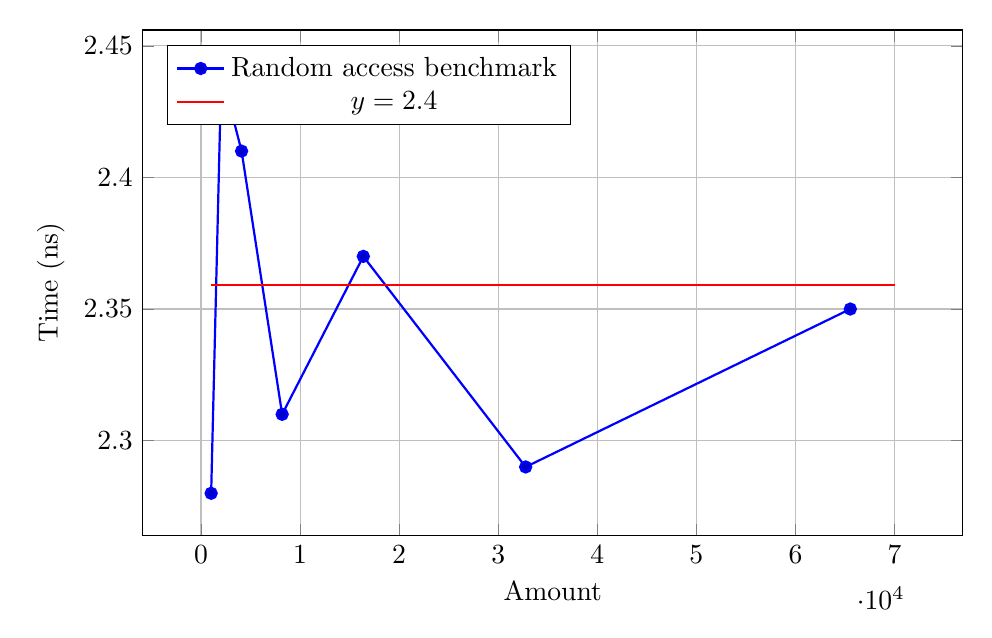
\begin{tikzpicture}
    \begin{axis}[
      xlabel={Amount},
      ylabel={Time (\si{\nano\second})},
      width=12cm, height=8cm,
      grid=major,
      legend pos=north west
    ]
      % Your benchmark data
      \addplot+[
        mark=*,
        thick,
        color=blue
      ] coordinates {
        (1024,   2.28)
        (2048,   2.44)
        (4096,   2.41)
        (8192,   2.31)
        (16384,  2.37)
        (32768,  2.29)
        (65536,  2.35)
      };
      \addlegendentry{Random access benchmark}

      \addplot[red, thick, domain=1000:70000] {2.359};
      \addlegendentry{$y = 2.4$}
      
    \end{axis}
  \end{tikzpicture}
  \caption{Random access benchmark with fitted line(s), x in array element size and y in time in nanoseconds}
  \label{fig:random-access}
\end{figure}


\section*{Array search benchmark}

Benchmarking array search is similar to benchmarking random array access, but the randomly generated keys are compared sequentially against each element of the array until a match is found or the end of the array is reached.

\begin{minted}{C}
  long search_benchmark(int n, int loop) {
    int *array = (int*) malloc(n*sizeof(int));
    for (int i = 0; i < n; i++)
        array[i] = rand()%(n*2);
    
    int *keys = (int*) malloc(loop*sizeof(int));
    for (int i = 0; i < loop; i++)
        keys[i] = rand()%(n*2);
    
    struct timespec t_start, t_stop;
    int sum = 0;
    clock_gettime(CLOCK_MONOTONIC, &t_start);
    for (int i = 0; i < loop; i++) {
        int key = keys[i];
        for (int j = 0; j < n; j++) {
            if (key == array[j]) {
                sum++;
                break;
            }
        }
    }
    clock_gettime(CLOCK_MONOTONIC, &t_stop);
    
    free(array);
    free(keys);
    
    long elapsed_time = nano_seconds(&t_start, &t_stop);
    return elapsed_time;
}
\end{minted}

In Table 2, judging the benchmark results, doubling the array size approximately doubles the execution time.

\begin{table}[h]
\begin{center}
\begin{tabular}{l|c}
\textbf{Size of array} & \textbf{Time per operation (amortized)}\\
\hline
  1024   &   1.7 µs   \\
  2048   &   3.3 µs   \\
  4096   &   6.4 µs   \\
  8192   &   13 µs    \\
  16384  &   26 µs    \\
  32768  &   51 µs    \\
  65536  &   100 µs   \\
  131072 &   200 µs   \\
\end{tabular}
\caption{Growing time in array search}
\label{tab:table1}
\end{center}
\end{table}

The fitted linear function in Figure 2 using least-squares regression in Figure 2 closely matches the measured data, with a small constant offset caused by loop overhead and control flow. This concludes that the time complexity of a linear array search is $ O(n) $, as the elapsed time grows linearly with the array size.

\begin{figure}
  \centering
  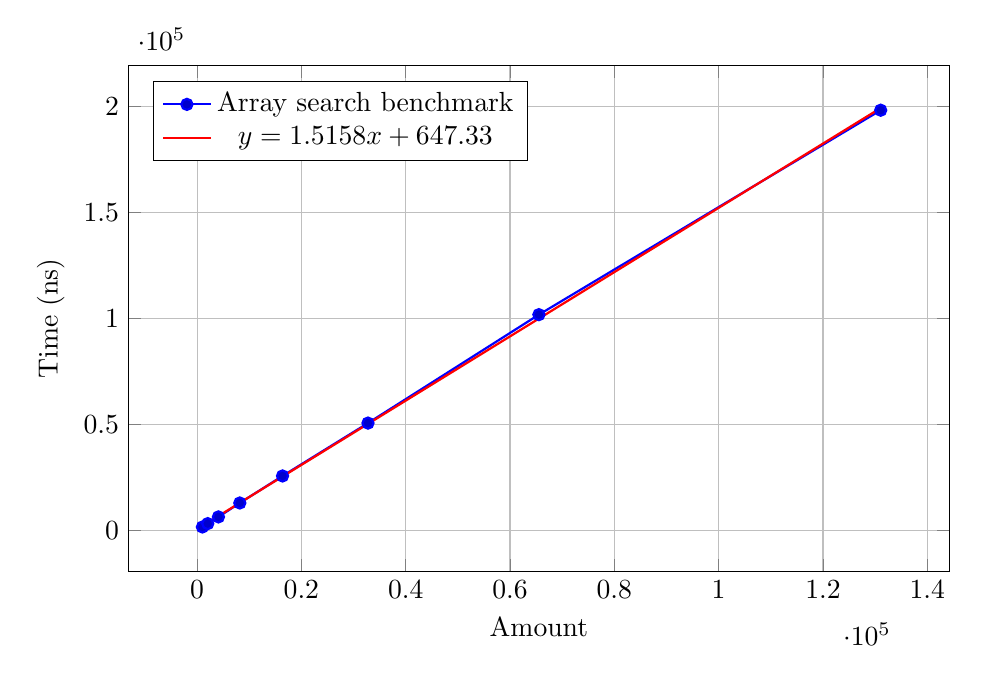
\begin{tikzpicture}
    \begin{axis}[
      xlabel={Amount},
      ylabel={Time (\si{\nano\second})},
      width=12cm, height=8cm,
      grid=major,
      legend pos=north west
    ]
      % Your benchmark data
      \addplot+[
        mark=*,
        thick,
        color=blue
      ] coordinates {
        (1024,   1679.10)
        (2048,   3268.07)
        (4096,   6436.80)
        (8192,   13010.31)
        (16384,  25751.70)
        (32768,  50693.34)
        (65536,  101850.42)
        (131072, 198295.30)
      };
      \addlegendentry{Array search benchmark}

      \addplot[red, thick, domain=0:131072] {1.5158*x + 647.33};
      \addlegendentry{$y = 1.5158x + 647.33$}
      
    \end{axis}
  \end{tikzpicture}
  \caption{Random access benchmark with fitted line(s)}
  \label{fig:random-access}
\end{figure}

\section*{Duplication}

Measuring the duplication algorithm, an array is first allocated on the heap, filled with random numbers.
The algorithm takes the array and checks for duplicates by iterating through each element in the array and comparing it with all subsequent elements. The algorithm begins with the first element in the array. If a duplicate is found, the inner loop is exited early. Otherwise, the next element becomes the comparing element and the process continues.

\begin{minted}{C}
  long duplicates_benchmark(int n) { 
      int *array = (int*) malloc(n*sizeof(int));
      for (int i = 0; i < n; i++)
          array[i] = rand()%(n*2);
      
      int sum = 0;
      struct timespec t_start, t_stop;
      
      clock_gettime(CLOCK_MONOTONIC, &t_start);
      for (int i = 0; i < n; i++) {
          int key = array[i];
          for (int j = i+1; j < n; j++) {
              if (key == array[j]) {
                  sum++;
                  break;
              }
          }
      }
      clock_gettime(CLOCK_MONOTONIC, &t_stop);
      
      free(array);
      
      return nano_seconds(&t_start, &t_stop);
  }
\end{minted}

In Table 3, the amortized time for each operation is roughly four times as large as the amount of elements in array doubles, by judging the benchmark result in time.

\begin{table}[h]
\begin{center}
\begin{tabular}{l|c}
\textbf{Size of array} & \textbf{Time (approximate)}\\
\hline
  1024   &  1.1 ms  \\  
  2048   &  3.7 ms  \\  
  4096   &  14 ms   \\ 
  8192   &  57 ms   \\ 
  16384  &  220 ms  \\  
  32768  &  890 ms  \\  
  65536  &  3.6 s   \\ 
  131072 &  14 s    \\
\end{tabular}
\caption{Quadratic time in array duplication checking algorithm}
\label{tab:table1}
\end{center}
\end{table}

Using least square-regression in figure 3, a quadratic time function produces a best fit to the given time measurements, with small linear and constant terms included in the model due to each loop overhead. As the array size increases, the term $ x^2 $ dominates in the fitted function, resulting into a $ O(n^2) $ time complexity.

\begin{figure}
  \centering
  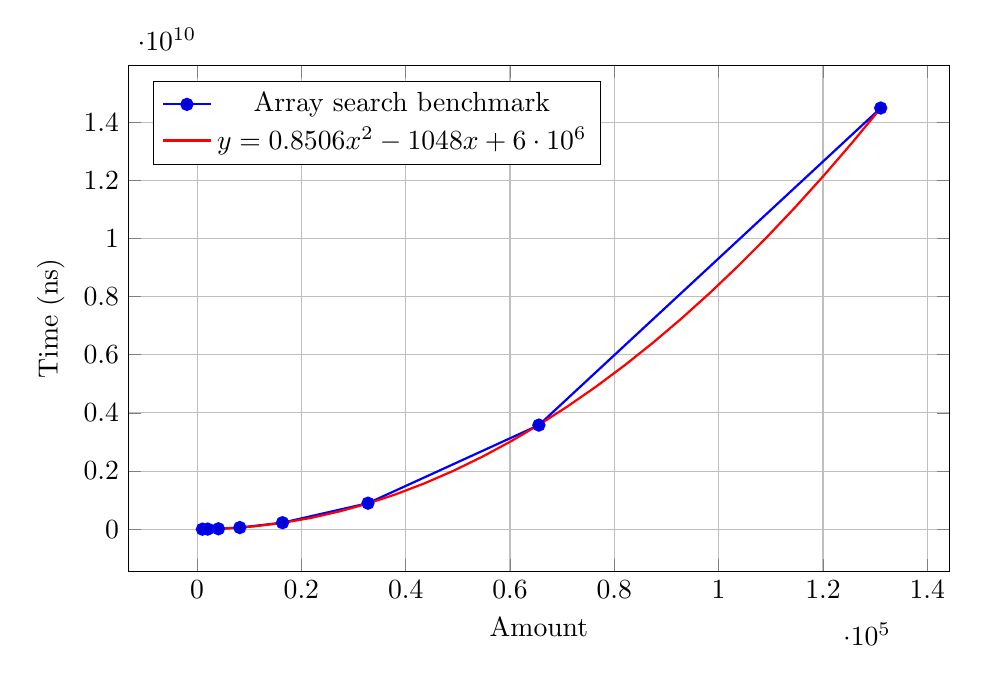
\begin{tikzpicture}
    \begin{axis}[
      xlabel={Amount},
      ylabel={Time (\si{\nano\second})},
      width=12cm, height=8cm,
      grid=major,
      legend pos=north west
    ]
      % Your benchmark data
      \addplot+[
        mark=*,
        thick,
        color=blue
      ] coordinates {
        (1024,   1065420.8)
        (2048,   3684608)
        (4096,   14206248.96)
        (8192,   56628264.96)
        (16384,  224418447.36)
        (32768,  894779381.76)
        (65536,  3580590469.12)
        (131072, 14484434739.2)
      };
      \addlegendentry{Array search benchmark}

      \addplot[red, thick, domain=0:131072] {0.8506*x^2 - 1048*x + 6e6};
      \addlegendentry{$y = 0.8506x^2 - 1048x + 6 \cdot 10^6$}
      
    \end{axis}
  \end{tikzpicture}
  \caption{Random access benchmark with fitted line(s)}
  \label{fig:random-access}
\end{figure}

\end{document}
